\documentclass[handout]{beamer}
\usefonttheme[onlymath]{serif}
\usepackage[T1]{fontenc}
\usepackage[utf8]{inputenc}
\usepackage[english, icelandic]{babel}
\usepackage{amsmath}
\usepackage{amssymb}
\usepackage{amsthm}
\usepackage{gensymb}
\usepackage{parskip}
\usepackage{mathtools}
\usepackage{listings}
\usepackage{xfrac}
\usepackage{graphicx}
\usepackage{xcolor}
\usepackage{tikz}
\usetikzlibrary{calc}
\usepackage{verbatim}
\usepackage{multicol}

\DeclareMathOperator{\lcm}{lcm}
\DeclareMathOperator{\diam}{diam}
\DeclareMathOperator{\dist}{dist}
\DeclareMathOperator{\ord}{ord}
\DeclareMathOperator{\Aut}{Aut}
\DeclareMathOperator{\Inn}{Inn}
\DeclareMathOperator{\Ker}{Ker}
\DeclareMathOperator{\trace}{trace}
\DeclareMathOperator{\fix}{fix}
\DeclareMathOperator{\Log}{Log}
\newcommand\floor[1]{\left\lfloor#1\right\rfloor}
\newcommand\ceil[1]{\left\lceil#1\right\rceil}
\newcommand\abs[1]{\left|#1\right|}
\newcommand\p[1]{\left(#1\right)}
\newcommand\sqp[1]{\left[#1\right]}
\newcommand\cp[1]{\left\{#1\right\}}
\newcommand\norm[1]{\left\lVert#1\right\rVert}
\renewcommand\qedsymbol{$\blacksquare$}
\renewcommand\Im{\operatorname{Im}}
\renewcommand\Re{\operatorname{Re}}
\usepackage{color}

\definecolor{mygray}{rgb}{0.4,0.4,0.4}
\definecolor{mygreen}{rgb}{0, 0, 1}
\definecolor{myorange}{rgb}{1.0,0.4,0}

\lstset{
commentstyle=\color{mygray},
numbersep=5pt,
numberstyle=\tiny\color{mygray},
keywordstyle=\color{mygreen},
showspaces=false,
showstringspaces=false,
stringstyle=\color{myorange},
tabsize=4
}
\lstset{literate=
{æ}{{\ae}}1
{í}{{\'{i}}}1
{ó}{{\'{o}}}1
{á}{{\'{a}}}1
{é}{{\'{e}}}1
{ú}{{\'{u}}}1
{ý}{{\'{y}}}1
{ð}{{\dh}}1
{þ}{{\th}}1
{ö}{{\"o}}1
{Á}{{\'{A}}}1
{Í}{{\'{I}}}1
{Ó}{{\'{O}}}1
{Ú}{{\'{U}}}1
{Æ}{{\AE}}1
{Ö}{{\"O}}1
{Ø}{{\O}}1
{Þ}{{\TH}}1
}

\usetheme{Madrid}

\title{Gagnagrindur}
\subtitle{\texttt{STL}, biltré, sammengisleit og rótarþáttun}
\author{Bergur Snorrason}
\date{\today}

\graphicspath{{myndir/}}

\AtBeginSection[] {
  \begin{frame}
    \frametitle{Efnisyfirlit}
    \tableofcontents[currentsection]
  \end{frame}
}

\begin{document}

\frame{\titlepage}

\section[STL]{STL}

\begin{frame}
\frametitle{STL}
\begin{itemize}
	\item<1-> Í flestum forritunarmálum eru ýmsar gagnagrindur útfærðar.
	\item<2-> Við köllum þessar gagnagrindur vanalega \texttt{STL}.
	\item<3-> Skoðum helstu \texttt{STL} gagnagrindur í \texttt{C++}.
\end{itemize}
\end{frame}

\begin{frame}
\frametitle{\texttt{vector}}
\begin{itemize}
	\item Gagnagrindin \texttt{vector} virkar svipað og fylki.
	\item Hún leyfir $\mathcal{O}(1)$ uppflettingu á $i$-ta stakinu.
	\item Hún leyfir $\mathcal{O}(1)$ breytingar á $i$-ta stakinu.
	\item Hún leyfir að skeyta staki aftast í $\mathcal{O}(1)$.
	\item Ef við getum gert eitthvað með fylki, þá getum við það líka með \texttt{vector}.
\end{itemize}
\end{frame}

\begin{frame}
\frametitle{Listi (\texttt{list})}
\begin{itemize}
	\item Gagnagrindin \texttt{list} er einteingdur listi.
	\item Við getum fundið $k$-ta stakið í lista í $\mathcal{O}(k)$.
	\item Við getum bætt við staki fyrir aftan gefið stak í $\mathcal{O}(1)$ (en þurfum fyrst að finna stakið).
	\item Við getum eytt staki fyrir aftan gefið stak í $\mathcal{O}(1)$ (en þurfum fyrst að finna stakið).
	\item Við getum skeytt saman listum í $\mathcal{O}(1)$.
\end{itemize}
\end{frame}

\begin{frame}
\frametitle{Hlaði (\texttt{stack})}
\begin{itemize}
	\item Gagnagrindin er mjög einföld.
	\item Við getum bætt við staki í $\mathcal{O}(1)$.
	\item Við getum fjarlægt/lesið stakið sem hefur verið styst í hlaðanum í $\mathcal{O}(1)$.
\end{itemize}
\end{frame}

\begin{frame}
\frametitle{Biðröð (\texttt{queue})}
\begin{itemize}
	\item Gagnagrindin er mjög einföld.
	\item Við getum bætt við staki í $\mathcal{O}(1)$.
	\item Við getum fjarlægt/lesið stakið sem hefur verið lengst í biðröðinni í $\mathcal{O}(1)$.
\end{itemize}
\end{frame}

\begin{frame}
\frametitle{\texttt{dequeue}}
\begin{itemize}
	\item Nafnið er stytting á ,,double-ended queue''.
	\item Við getum skeytt staki fremst eða aftast í $\mathcal{O}(1)$.
	\item Við getum fjarlægt/lesið stakið fremst eða aftast í $\mathcal{O}(1)$.
\end{itemize}
\end{frame}

\begin{frame}
\frametitle{Forgangsbiðröð (\texttt{prioirit\_queue})}
\begin{itemize}
	\item Gagnagrindin geymir samanberanleg stök.
	\item Gerum ráð fyrir sambanburður stakana taki $k$ tíma og það séu $n$ stök í biðröðinni.
	\item Við getum bætt við stökum í $\mathcal{O}(k \log n)$.
	\item Við getum fjarlægt stakið með hæstan forgang í $\mathcal{O}(k \log n)$.
	\item Við getum lesið stakið með hæstan forgang í $\mathcal{O}(1)$.
\end{itemize}
\end{frame}

\begin{frame}
\frametitle{Mengi (\texttt{set})}
\begin{itemize}
	\item Gagnagrindin geymir samanberanleg stök.
	\item Gerum ráð fyrir sambanburður stakana taki $k$ tíma og það séu $n$ stök í menginu.
	\item Við getum bætt við staki í mengið í $\mathcal{O}(k \log n)$.
	\item Við getum fjarlægt stak úr menginu í $\mathcal{O}(k \log n)$.
	\item Við getum athugað hvort stak sé í menginu í $\mathcal{O}(k \log n)$.
	\item Einnig er til \texttt{multiset}, sem leyfir endurtekningar.
\end{itemize}
\end{frame}

\section[Hrúgur]{Hrúgur}

\begin{frame}
\frametitle{Hrúgur}
\begin{itemize}
	\item<1-> Rótartvíundatré sem uppfyllir að sérhver nóða er stærri en börnin sín er sagt uppfylla \emph{hrúguskilyrðið}.
	\item<2-> Við köllum slík tré \emph{hrúgur} (e. heap).
	\item<3-> Hrúgur eru heppilega auðveldar í útfærslu.
	\item<4-> Við geymum tréð sem fylki og eina erfiðið er að viðhalda hrúguskilyrðinu.
\end{itemize}
\end{frame}

\begin{frame}
\frametitle{Fylki sem tré}
\begin{itemize}
\item<1-> Þegar við geymum tréð sem fylki notum við eina af tveimur aðferðum.
\item<2-> Sú fyrri:
	\begin{itemize}
		\item<3-> Rótin er í staki $1$ í fylkinu.
		\item<4-> Vinstra barn staksins $i$ er stak $2\times i$.
		\item<5-> Hægra barn staksins $i$ er stak $2\times i + 1$.
		\item<6-> Foreldri staks $i$ er stakið $\left \lfloor \dfrac{i}{2} \right \rfloor$.
	\end{itemize}
\item<7-> Sú seinni:
	\begin{itemize}
		\item<8-> Rótin er í staki $0$ í fylkinu.
		\item<9-> Vinstra barn staksins $i$ er stak $2\times i + 1$.
		\item<10-> Hægra barn staksins $i$ er stak $2\times i + 2$.
		\item<11-> Foreldri staks $i$ er stakið $\left \lfloor \dfrac{i - 1}{2} \right \rfloor$.
	\end{itemize}
\end{itemize}
\end{frame}

\begin{frame}[fragile]
	\frametitle{Hrúga í \texttt{C}}
	\tiny
	\begin{lstlisting}[language=C]
#define PARENT(i) ((i - 1)/2)
#define LEFT(i)   ((i)*2 + 1)
#define RIGHT(i)  ((i)*2 + 2)
int h[1000000];
int hn = 0;

void fix_down(int i)
{
	...
}

void fix_up(int i)
{
	...
}

void pop()
{
	...
}

int peek()
{
	...
}

void push(int x)
{
	...
}
\end{lstlisting}
\end{frame}

\begin{frame}[fragile]
	\frametitle{Hrúga í \texttt{C}}
	\tiny
	\begin{lstlisting}[language=C]
void pop()
{
	hn--;
	h[0] = h[hn];
	fix_down(0);
}

int peek()
{
	return h[0];
}

void push(int x)
{
	h[hn++] = x;
	fix_up(hn - 1);
}
\end{lstlisting}
\end{frame}

\begin{frame}[fragile]
	\frametitle{Hrúga í \texttt{C}}
	\tiny
	\begin{lstlisting}[language=C]
void fix_down(int i)
{
	int mx = i;
	if (RIGHT(i) < hn && h[mx] < h[RIGHT(i)]) mx = RIGHT(i);
	if (LEFT(i) < hn && h[mx] < h[LEFT(i)]) mx = LEFT(i);
	if (mx != i)
	{
		swap(h[i], h[mx]);
		fix_down(mx);
	}
}
\end{lstlisting}
\end{frame}

\begin{frame}[fragile]
	\frametitle{Hrúga í \texttt{C}}
	\tiny
	\begin{lstlisting}[language=C]
void fix_up(int i)
{
	if (i == 0) return;
	else if (h[i] > h[PARENT(i)])
	{
		swap(h[i], h[PARENT(i)]);
		fix_up(PARENT(i));
	}
}
\end{lstlisting}
\end{frame}

\section[Biltré]{Biltré}

\begin{frame}
\frametitle{Dæmi}
\begin{itemize}
\item<1-> Gefinn er listi með $n$ tölum.
\item<2-> Næst koma $q$ fyrir spurnir, þar sem hver er af einni af tveimur gerðum:
	\begin{itemize}
	\item<3-> Breyttu $i$-tu tölunni í listanum í $k$.
	\item<4-> Reiknaðu summu allra talna á bilinu $[i, j]$.
	\end{itemize}
\item<5-> Það er auðséð að einföld útfærlsa á þessum fyrir spurnum gefur okkur $\mathcal{O}(1)$ fyrir þá fyrri og $\mathcal{O}(n)$ fyrir þá seinni.
\item<6-> Þar sem allar (eða langflestar) fyrirspurnir gætu verið af seinni gerðin yrði lausnin í heildin $\mathcal{O}(qn)$.
\item<7-> Það er þó hægt að leysa þetta dæmi hraðar.
\item<8-> Algengt er að nota til þess \emph{biltré}.
\end{itemize}
\end{frame}

\begin{frame}
\frametitle{Biltré}
\begin{itemize}
\item<1-> Biltré (e. segment tree) er tvíundartré sem geymir svör við vissum fyrirspurnum af seinni gerðinni.
\item<2-> Rótin geymir svar við fyrirspurninni \texttt{1 n} 
og ef nóða geymir svarið við \texttt{i j} þá geyma börn hennar svör við \texttt{i m} og \texttt{m + 1 j}, þar sem $m$ er miðja heiltölubilsins $[i, j]$.
\item<3-> Þær nóður sem geyma svar við fyrirspurnum af gerðinni \texttt{i i} eru lauf trésins.
\end{itemize}
\end{frame}

\begin{frame}
\frametitle{Mynd af biltré, $n = 4$}
	\begin{figure}
		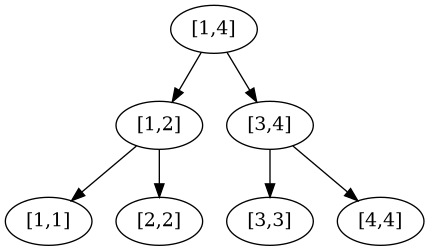
\includegraphics[scale=0.5]{mynd2.png}
	\end{figure}
\end{frame}

\begin{frame}
\frametitle{Mynd af biltré, $n = 7$}
	\begin{figure}
		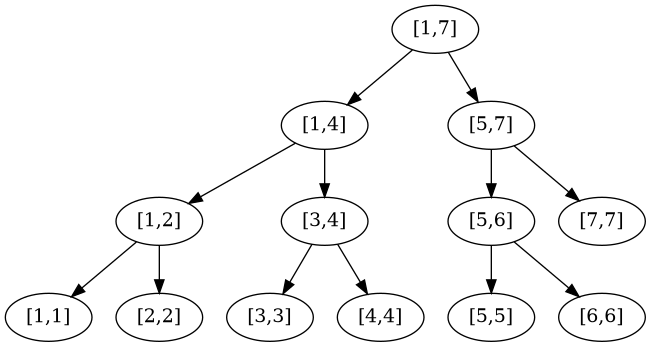
\includegraphics[scale=0.3]{mynd3.png}
	\end{figure}
\end{frame}

\begin{frame}
\frametitle{Notkun biltrjáa}
\begin{itemize}
\item<1-> Gerum ráð fyrir að við höfum biltré eins og lýst er að ofan og látum $H$ tákna hæð trésins.
\item<2-> Hvernig getum við leyst fyrirspurnirnar á glærunni á undan, og hver er tímaflækjan?
\item<3-> Fyrri fyrirspurnin er einföld.
\item<4-> Ef við eigum að breyta $i$-ta stakinu í $k$ finnum við fyrst laufið sem svarar til fyrirspurnar \texttt{i i},
	setjum svarið þar sem $k$ og förum svo upp í rót í gegnum foreldrana og uppfærum á leiðinni gildin í þeim nóðu sem við lendum í.
\item<5-> Þar sem við heimsækjum bara þær nóður sem eru á veginum frá rót til laufs (mest $H$ nóður) er tímaflækjan á fyrri fyrirspurninn $\mathcal{O}(H)$.
\end{itemize}
\end{frame}

\begin{frame}[fragile]
	\frametitle{Biltré í \texttt{C}}
	\tiny
	\begin{lstlisting}[language=C]
// ath: p er af staerd 4*n + 1
#define LEFT(x) ((x)*2)
#define RIGHT(x) ((x)*2 + 1)
void update(int* p, int i, int j, int x, int y, int e)
{
	if (i == j) p[e] = y;
	else
	{
		int m = (i + j)/2;
		if (x <= m) update(p, i, m, x, y, LEFT(e));
		else update(p, m + 1, j, x, y, RIGHT(e));
		p[e] = p[LEFT(e)] + p[RIGHT(e)];
	}
}
\end{lstlisting}
\end{frame}

\begin{frame}
\frametitle{Notkun biltrjáa}
\begin{itemize}
\item<1-> Seinni fyrirspurnin er ögn flóknari.
\item<2-> Auðveldast er að ímynda sér að við förum niður tréð og leitum að hvorum endapunktinum fyrir sig.
\item<3-> Á leiðinni upp getum við svo pússlað saman svarinu, eftir því hvort við erum að skoða hægri eða vinstri endapunktinn.
\item<4-> Til dæmis, ef við erum að leita að vinstri endapunkti $x$ og komum upp í bil $[i, j]$ þá bætum við gildinu í nóðu
$[i, m]$ við það sem við höfum reiknað hingað til ef $x \in [m + 1, j]$, en annars bætum við engu við (því $x$ er vinstri endapunkturinn).
\item<5-> Við göngum svona upp þar til við lendum í bili sem inniheldur hinn endapunktinn.
\item<6-> Með sömu rökum og áðan er tímaflækjan $\mathcal{O}(H)$.
\end{itemize}
\end{frame}

\begin{frame}[fragile]
	\frametitle{Biltré í \texttt{C}}
	\tiny
	\begin{lstlisting}[language=C]
int queryl(int* p, int i, int j, int x, int e)
{
	if (i == j) return p[e];
	int m = (i + j)/2;
	return (x <= m) ? (queryl(p, i, m, x, LEFT(e)) + p[RIGHT(e)])
                    : (queryl(p, m + 1, j, x, RIGHT(e)));
}

int queryr(int* p, int i, int j, int x, int e)
{
	if (i == j) return p[e];
	int m = (i + j)/2;
	return (x <= m) ? (queryr(p, i, m, x, LEFT(e)))
                    : (p[LEFT(e)] + queryr(p, m + 1, j, x, RIGHT(e)));
}

int query(int* p, int i, int j, int x, int y, int e)
{
	if (i == j) return p[e];
	int m = (i + j)/2;
	if (x <= m && y <= m) return query(p, i, m, x, y, LEFT(e));
	if (x > m && y > m) return query(p, m + 1, j, x, y, RIGHT(e));
	return queryl(p, i, m, x, LEFT(e)) + queryr(p, m + 1, j, y, RIGHT(e));
}
\end{lstlisting}
\end{frame}

\begin{frame}
\frametitle{Tímaflækja biltrjáa}
\begin{itemize}
\item<1-> Þar sem lengd hvers bils sem nóða svara til helmingast þegar farið er niður tréð er $\mathcal{O}(H) = \mathcal{O}(\log n)$.
\item<2-> Við erum því komin með lausn á upprunalega dæminu sem er $\mathcal{O}(q \log n)$.
\item<3-> Þetta væri nógu hratt ef, til dæmis, $n = q = 10^5$.
\end{itemize}
\end{frame}

\begin{frame}
\frametitle{Annað dæmi}
\begin{itemize}
\item<1-> Fyrsta lína inntaksins inniheldur tvær tölur, $n$ og $m$, báðar jákvæðar heiltölur minni en $10^5$.
\item<2-> Næsta lína inniheldur $n$ heiltölur, á milli $-10^9$ og $10^9$.
\item<3-> Næstu $m$ línur innihalda fyrirspurnir, af tveimur gerðum. 
\item<4-> Fyrri gerðin hefst á \texttt{1} og inniheldur svo tvær tölur, $x$ og $y$. Hér á að setja $x$-tu töluna sem $y$.
\item<5-> Seinni gerðin hefst á \texttt{2} og inniheldur svo tvær tölu,
$x$ og $y$. Hér á að prenta út stærstu töluna á hlutbilinu $[x, y]$ í talnalistanum.
\item<6-> Hvernig leysum við þettta?
\end{itemize}
\end{frame}

\begin{frame}[fragile]
	\frametitle{Lausn}
	\tiny
	\begin{lstlisting}[language=C]
int queryl(int* p, int i, int j, int x, int e)
{
	if (i == j) return p[e];
	int m = (i + j)/2;
	return (x <= m) ? (max(queryl(p, i, m, x, LEFT(e)), p[RIGHT(e)]))
                    : (queryl(p, m + 1, j, x, RIGHT(e)));
}
int queryr(int* p, int i, int j, int x, int e)
{
	if (i == j) return p[e];
	int m = (i + j)/2;
	return (x <= m) ? (queryr(p, i, m, x, LEFT(e)))
                    : (max(p[LEFT(e)], queryr(p, m + 1, j, x, RIGHT(e))));
}
int query(int* p, int i, int j, int x, int y, int e)
{
	if (i == j) return p[e];
	int m = (i + j)/2;
	if (x <= m && y <= m) return query(p, i, m, x, y, LEFT(e));
	if (x > m && y > m) return query(p, m + 1, j, x, y, RIGHT(e));
	return max(queryl(p, i, m, x, LEFT(e)), queryr(p, m + 1, j, y, RIGHT(e)));
}
void update(int* p, int i, int j, int x, int y, int e)
{
	if (i == j) p[e] = y;
	else
	{
		int m = (i + j)/2;
		if (x <= m) update(p, i, m, x, y, LEFT(e));
		else update(p, m + 1, j, x, y, RIGHT(e));
		p[e] = max(p[LEFT(e)], p[RIGHT(e)]);
	}
}
	\end{lstlisting}
\end{frame}

\begin{frame}[fragile]
	\frametitle{Lausn}
	\tiny
	\begin{lstlisting}[language=C]
int main()
{
	int n, m, i, x, y, z;
	scanf("%d%d", &n, &m);
	int a[n], p[4*n + 1];
	for (i = 0; i < n; i++) scanf("%d", &(a[i]));
	for (i = 0; i < 4*n + 1; i++) p[i] = 0;
	for (i = 0; i < n; i++) update(p, 0, n - 1, i, a[i], 1);
	while (m-- != 0)
	{
		scanf("%d%d%d", &x, &y, &z);
		if (x == 1) update(p, 0, n - 1, y, z, 1);
		if (x == 2) printf("%d\n", query(p, 0, n - 1, y, z, 1));
	}

	return 0;
}
	\end{lstlisting}
\end{frame}

\begin{frame}[fragile]
	\frametitle{Betri útfærsla}
	\tiny
Atli fann þessa stuttu og snyrtilegu útfærslu.\\
ATH: Bilið í query er núna hálfopið.
	\begin{lstlisting}[language=C]
#include<bits/stdc++.h>
using namespace std;
typedef vector<int> vi;

struct segtree {
    int n; vi d; 
    segtree(vi o) : n(o.size()), d(2 * o.size()) {
        for(int i = 0; i < n; ++i) d[n + i] = o[i];
        for(int i = n - 1; i > 0; --i) d[i] = d[i << 1] + d[i << 1|1];
    }
    void update(int at, int by) {
        for(d[at += n] = by; at > 1; at >>= 1) d[at >> 1] = d[at] + d[at ^ 1];
    }
    int query(int l, int r) { // [l, r[
        int res = 0;
        for(l += n, r += n; l < r; l >>= 1, r >>= 1) {
            if(l & 1) res += d[l++];
            if(r & 1) res += d[--r];
        }
        return res;
    }
};

int main() {
    vi tst = {0, 1, 2, 3, 4, 5, 6};
    segtree st(tst);
    cout << st.query(0, 3) << endl;
    st.update(1, 4);
    cout << st.query(1, 3) << endl;
}
	\end{lstlisting}
\end{frame}

\section[Sammengisleit]{Sammengisleit}

\begin{frame}
\frametitle{Sammengisleit}
\begin{itemize}

\item<1-> Sammengisleit (e. union-find) er öflug leið til að halda utan um jafngildisflokka tiltekna vensla,
	eða m.ö.o. halda utan um \emph{sundurlæg} mengi.
\item<2-> Við viljum getað:
	\begin{itemize}
		\item<3-> Borið saman samhengisþætti mismunandi staka.
		\item<4-> Sameinað samhengisflokka.
	\end{itemize}
\item<5-> Við tölum um aðgerðirnar \texttt{find(x)} og \texttt{join(x, y)}.

\end{itemize}
\end{frame}

\begin{frame}
\frametitle{Dæmi}
\begin{itemize}

	\item<1-> Tökum sem dæmi einstökungasafnið
		$\{\{1\}, \{2\}, \{3\}, \{4\}, \{5\}\}$. 
	\item<2-> \texttt{join(1, 3)} gefur okkur
		$\{\{1, 3\}, \{2\}, \{4\}, \{5\}\}$. 
	\item<3-> \texttt{join(2, 5)} gefur okkur
		$\{\{1, 3\}, \{2, 5\}, \{4\}\}$. 
	\item<4-> \texttt{join(2, 4)} gefur okkur
		$\{\{1, 3\}, \{2, 4, 5\}\}$. 
	\item<5-> \texttt{join(1, 4)} gefur okkur
		$\{\{1, 2, 3, 4, 5\}\}$. 
	\item<6-> Á sérhverjum tímapunkti myndi \texttt{find(x)} skila einhverju staki sem er í sama mengi og \texttt{x}.
	\item<7-> Aðalatriðið er að \texttt{find(x)} skilar sama stakinu fyrir sérhvert stak í sérhverjum samhengisflokki.
	\item<8-> Til dæmis, í þriðja punktinum myndi \texttt{find(1)} og \texttt{find(3)} alltaf skila sama stakinu.
\end{itemize}
\end{frame}

\begin{frame}
\frametitle{Útfærsla á frumstæðri sammengisleit}
\begin{itemize}
	\item<1-> Gerum ráð fyrir að tölurnar sem við munum vinna með séu jákvæðar og minni en $n$.
	\item<2-> Við munum þá gefa okkur $n$ staka fylki $p$, þar sem $i$-ta stakið í fylkinu er upphafstillt sem $i$.
	\item<3-> Fylkið $p$ mun nú geyma \emph{foreldri} sérhvers stak.
	\item<4-> Foreldrin myndi keðjur.
	\item<5-> Sérhver keðja endar í einhverju staki, sem við munum kalla \emph{ráðherra} jafngildisflokksins.
\end{itemize}
\end{frame}

\begin{frame}
\frametitle{Mynd af keðjum}
	Keðjurnar sem fást með $\{\{0, 2, 4, 5, 9, 10\}, \{1, 3, 6, 11\}, \{7, 8\}\}$ gætu til dæmis verið
	gefnar með $p = [0, 1, 0, 1, 0, 4, 3, 7, 7, 5, 5, 3]$.
	\begin{figure}
	\item<2->
		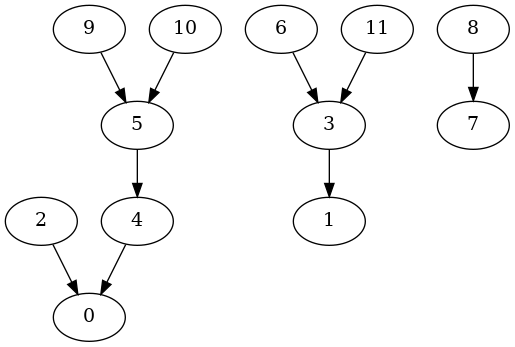
\includegraphics[scale=0.5]{mynd.png}
	\end{figure}
\end{frame}

\begin{frame}
\frametitle{Útfærsla á frumstæðri sammengisleit}
\begin{itemize}
	\item<1-> Til að fá ráðherra flokks tiltekins staks er hægt að fara endurkvæmt upp keðjuna.
	\item<2-> Til að sameina flokka nægir að breyta foreldri ráðherra annars flokksins yfir í
		eitthvert stak hins flokksins (sér í lagi ráðherra þess).
	\item<3-> Báðar þessar aðgerðir er auðvelt að útfæra.
\end{itemize}
\end{frame}

\begin{frame}[fragile]
	\frametitle{Frumstæð sammengisleit}
\tiny
\begin{lstlisting}[language=C++]
int p[MAX];

int find(int x)
{
	if (p[x] == x) return x;
	return find(p[x]);
}

void join(int x, int y)
{
	p[find(x)] = find(y);
}

int main()
{
	int i;
	int n = MAX;
	for (i = 0; i < n; i++) p[i] = i;
	...
}
\end{lstlisting}
\end{frame}

\begin{frame}
\frametitle{Tímaflækjur frumstæðri sammengisleitar}
\begin{itemize}
	\item<1-> Við sjáum nú að tímaflækja \texttt{find} er línuleg í lengd keðjunnar, svo 
		þar sem lengd keðjunnar getur verið í versta falli $n$ þá er \texttt{find} $\mathcal{O}(n)$.
	\item<2-> Fallið \texttt{join} gerir lítið annað en að kalla tvisvar á \texttt{find} svo það er líka
		$\mathcal{O}(n)$.
	\item<3-> Er samt ekki hægt að bæta þetta eitthvað?
	\item<4-> Það er vissulega hægt!
\end{itemize}
\end{frame}

\begin{frame}
\frametitle{Keðjuþjöppuð sammengisleit}
\begin{itemize}
	\item<1-> Eins og nafnið á glærunni gefur til kynna er hugmyndin að þjappa keðjunum saman í hvert skipti sem kallað er á
		\texttt{find}.
	\item<2-> Þetta er gert með því að setja \texttt{p[x]} sem ráðherra flokks \texttt{x}, í hverju skrefi endurkvæmninnar.
\end{itemize}
\end{frame}

\begin{frame}
\frametitle{Dæmi um keðjuþjöppun}
\begin{itemize}
	\item<1-> Gefum okkur
		$p = [0, 0, 1, 2, 3, 4, 5, 6, 7]$.
	\item<2-> Ljóst er að \texttt{find(5)} skilar $0$.
	\item<3-> Ef við notum frumstæða sammengisleit breytist $p$ ekki neitt þegar kallað er á \texttt{find}
		en með keðjuþjappaðri sammengisleit þjappast keðjan frá og með $5$ og því fæst
		$p = [0, 0, 0, 0, 0, 0, 5, 6, 7]$.
\end{itemize}
\end{frame}

\begin{frame}[fragile]
	\frametitle{Keðjuþjöppað sammengisleit}
\tiny
\begin{lstlisting}[language=C++]
int p[MAX];

int find(int x)
{
	if (p[x] == x) return x;
	return p[x] = find(p[x]);
}

void join(int x, int y)
{
	p[find(x)] = find(y);
}

int main()
{
	int i;
	int n = MAX;
	for (i = 0; i < n; i++) p[i] = i;
	...
}
\end{lstlisting}
\end{frame}

\begin{frame}
\frametitle{Tímaflækjur keðjuþjappaðar sammengisleitar}
\begin{itemize}
	\item<1-> Það er flóknara að lýsa tímaflækju keðjuþjappaðrar sammengisleitar.
	\item<2-> \emph{Á heildina litið} (e. amortized) er tímaflækjan er $\mathcal{O}(\alpha(n))$, þar sem $\alpha$ er andhverfa \emph{Ackermann} fallsins.
	\item<3-> Fyrir þau $n$ sem við fáumst við er $\alpha(n)$ nánast fast.
\end{itemize}
\end{frame}

\section[Rótarþáttun]{Rótarþáttun}

\begin{frame}
\frametitle{Rótarþáttun}
\begin{itemize}
	\item<1-> Skoðum aftur dæmið sem við skoðuðum í biltrjáa kaflanum.
	\item<2-> Hvað ef við skiptum listanum okkar upp í nokkurn hólf og geymum summu hvers hólfs fyrir sig.
	\item<3-> Segjum að við höfum $k$ hólf, og $n$ tölur.
	\item<4-> Ef við viljum finna summu yfir hlutbil nægir okkur leggja saman þau gildi frá endapunktum bilsins upp að næstu hólfamörkum,
		svo leggjum við saman hólfin á milli.
	\item<5-> Þessa aðgerð er því $\mathcal{O}(k + n/k)$, og ef við veljum $k = \sqrt{n}$ fæst að hún er $\mathcal{O}(\sqrt{n})$.
	\item<6-> Til að uppfæra gildi í listanum leggjum við saman öll stökin í hólfinu, sem tekur $\mathcal{O}(\sqrt{n})$.
\end{itemize}
\end{frame}

\begin{frame}
\frametitle{Rótarþáttun}
\begin{itemize}
	\item<1-> Þessa almennu aðferð má nota í flestum dæmum sem eru leysanleg með biltrjám og kallast hún \emph{rótarþáttun} (e. squareroot decomposition).
	\item<2-> Þetta er þó hægara en biltréin (virkar t.d. ekki fyrir $n = 10^6$.
	\item<3-> Kosturinn við þessa aðferð er að hún er létt í útfærlsu eftir smá æfingu og er almennari en biltréin.
\end{itemize}
\end{frame}

\begin{frame}[fragile]
	\frametitle{Rótarþáttun}
\tiny
\begin{lstlisting}[language=C++]
#include <stdio.h>
int main()
{
	int n, m, i, x, y, z, k = 1;
	scanf("%d%d", &n, &m);
	while (k*k < n) k++;
	int a[n], b[k];
	for (i = 0; i < n; i++) scanf("%d", &(a[i]));
	for (i = k; i < k; i++) b[i] = 0;
	for (i = 0; i < n; i++) b[i/k] += a[i];
	while (m-- != 0)
	{
		scanf("%d%d%d", &x, &y, &z);
		if (x == 1)
		{
			b[y/k] = b[y/k] - a[y] + z;
			a[y] = z;
		}
		if (x == 2)
		{
			int r = 0, k1 = y/k, k2 = z/k;
			if (k2 - k1 < 2) for (i = y; i <= z; i++) r += a[i];
			else
			{
				while (y/k == k1) r += a[y++];
				while (z/k == k2) r += a[z--];
				for (i = k1 + 1; i < k2; i++) r += b[i];
			}
			printf("%d\n", r);
		}
	}
	return 0;
}
\end{lstlisting}
\end{frame}

\end{document}
